%\clearpage
\section{AS-level topology}
\label{sec:as}

When trying to establish a precise meaning or interpretation of the use of 
``Internet topology,'' in much of the existing literature, we find that the 
phrase has often been taken to mean a virtual construct or graph created by 
the Border Gateway Protocol (BGP) routing protocol.  Commonly referred to as 
the inter-domain or Autonomous-System (AS) topology --- named after the logical 
blocks (ASes) that are used in BGP to designate the origin and path of routing 
announcements --- it is this particular connectivity structure that we focus 
on in this section, though we will see that the notion of the AS-topology is 
more slippery than commonly imagined. In particular, we will discuss some of 
the main issues that arise in the context of studying the Internet's AS topology 
(ranging from proper definitions and interpretations of this construct to 
measurements) and focus less on modeling-related aspects as they are still in
their infancy, especially when compared to the advances in router-topology
modeling described in \autoref{sec:router}.


\subsection{A look back}
\label{sec:as_hist}

As far as we know, the first researchers to use BGP-based measurements
in the form of route monitor data for topology-related work were
Govindan and Reddy~\cite{govindan97:_topology}, who introduced the
notion of the {\em inter-domain topology} defined as ``the graph of
domains and the inter-domain peering relationships.''  However,
although they were quite specific in regard to being interested in
routing, the concept was reused when
Faloutsos~\etal~\cite{faloutsos99:_power_law_relat_of_inter_topol}
coined the term ``Internet topology'', a paper that is more widely
cited (at least outside of the network research literature)
than~\cite{govindan97:_topology}.  The
paper~\cite{faloutsos99:_power_law_relat_of_inter_topol} is
responsible for advancing the alluring notion that the inter-domain
topology of the Internet is a well-defined object and can be {\em
  accurately} obtained and reconstructed from the available BGP route
monitor data. As we shall see, this is not at all the case, and it has
fed into a large subsequent scientific literature, already discussed
earlier, \eg \cite{barabasi99,barabasi02}.

The problems lie in the very definitions of the AS-topology and the
measurements that have been used to study this topology (we return to
the measurements in \autoref{sec:as_measurement} below).  In terms of
definitions, in the context of the AS-level Internet, it is tempting
to simply equate a node with an AS, but this begs the question what an
AS really is.  The term refers formally to the AS number (ASN)
allocated by IANA (Internet Assigned Numbers Authority) or the
Regional Internet Registries (RIRs). An ASN is tendered to enable
routing using BGP.  This is {\bf not} equivalent to the popular view
that associates an AS with a set of routers that appear to the outside
as if they formed a single coherent system with a 1:1 mapping between
it and some administering company.

For instance, an organization may often own a router which has at least one 
interface IP address belonging to another organization. In fact, many point-to-point 
IP links occur across a ``/30'' subnet. When the link joins two networks, this subnet 
must be allocated from the IP blocks of one or the other connecting network, and so 
most such connections result in IP addresses from neighboring ASes appearing locally. 

Another problem arises from the fact that although an AS is often considered to 
correspond to a single technical administrative domain, \ie a network run by one 
organization, it is common practice for a single organization to manage multiple 
ASes, each with their own ASN~\cite{cai10:_AS_to_organ_map}. For instance, Verizon 
Business (formerly known as UUNET) uses ASNs 701, 702, 703 to separate its
E-BGP network into three geographic regions, but runs a single IGP instance throughout 
its whole network. In terms of defining nodes of a graph, these three networks are all 
under the same operational administrative control, and hence should be viewed as a 
single node. On the other hand, as far as ASNs are concerned, they are different and 
should be treated as three separate nodes.  The situation is actually more complex 
since corporations like Verizon Business own some 200+ ASNs~\cite{cai10:_AS_to_organ_map} 
(not all are actually used, though). In many of these cases, a clear boundary between 
these multiple ASes may not really exist, thus blurring the definition of
the meaning of a node in an AS graph. Similar problems can arise when a single AS 
is managed by multiple administrative authorities which consist of individuals 
from different corporations. For example, AS 2914 is run partially by NTT/America 
and partially by NTT/Asia.

All this presumes that an AS is a uniform, contiguous entity, but that
is not necessarily
true~\cite{muehlbauer06:_build_as,muehlbauer07:_in_search}. An AS may
very well announce different sets of prefixes at different exit points
of its network, or use BGP to balance traffic across overloaded links
(other reasons for heterogeneous configurations are reported
in~\cite{bush09:_inter_optom}). \autoref{fig:puzzle} illustrates the
problem. The AS-graph simplifies, in some cases grossly, the very
complicated structure of the entities involved, which are often
heterogeneous, and not necessarily even contiguous either
geographically or logically.

For all these reasons, it should be clear that modeling an AS as a single 
{\em atomic} node without internal (or external) structure is overly simplistic 
for most practical problems. Moreover, these issues cannot simply be addressed 
by moving towards graph representations that can account for some internal 
node structure (such as in~\cite{muehlbauer06:_build_as}), mainly because 
BGP is unlikely to reveal sufficient information to infer the internal structure 
for the purpose of faithful modeling.

\begin{figure}[!th] 
  \begin{center}
    \begin{subfigure}[b]{0.34\textwidth}
      \centering 
      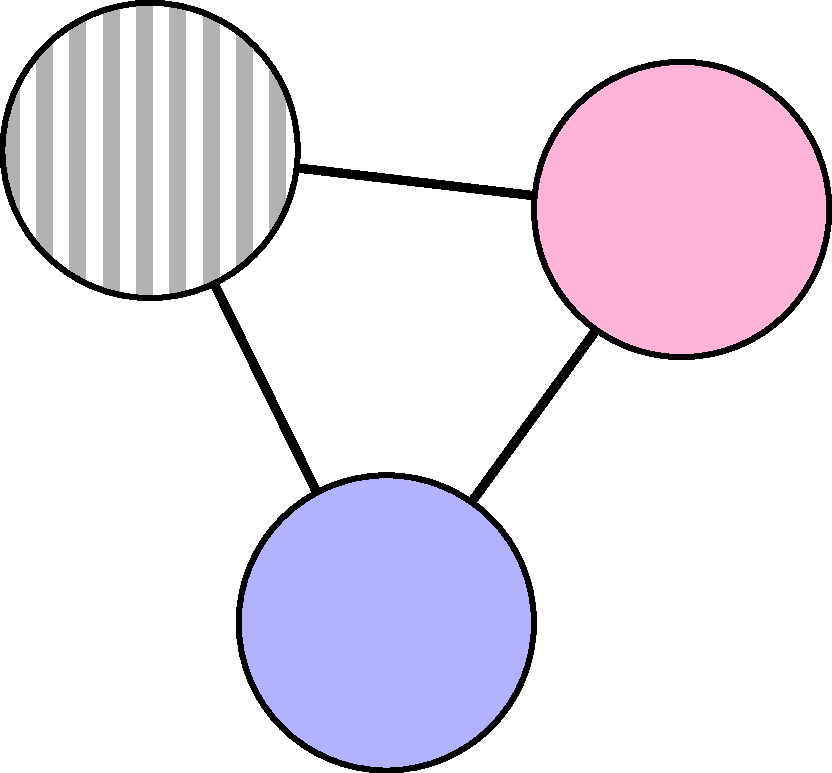
\includegraphics[width=1\textwidth]{puzzle_1.pdf}
      \vspace{17mm}
      \caption{A simple section of the ``AS-graph''.}
    \end{subfigure}
    \hspace{0.05\textwidth}
    \begin{subfigure}[b]{0.54\textwidth}
      \centering
      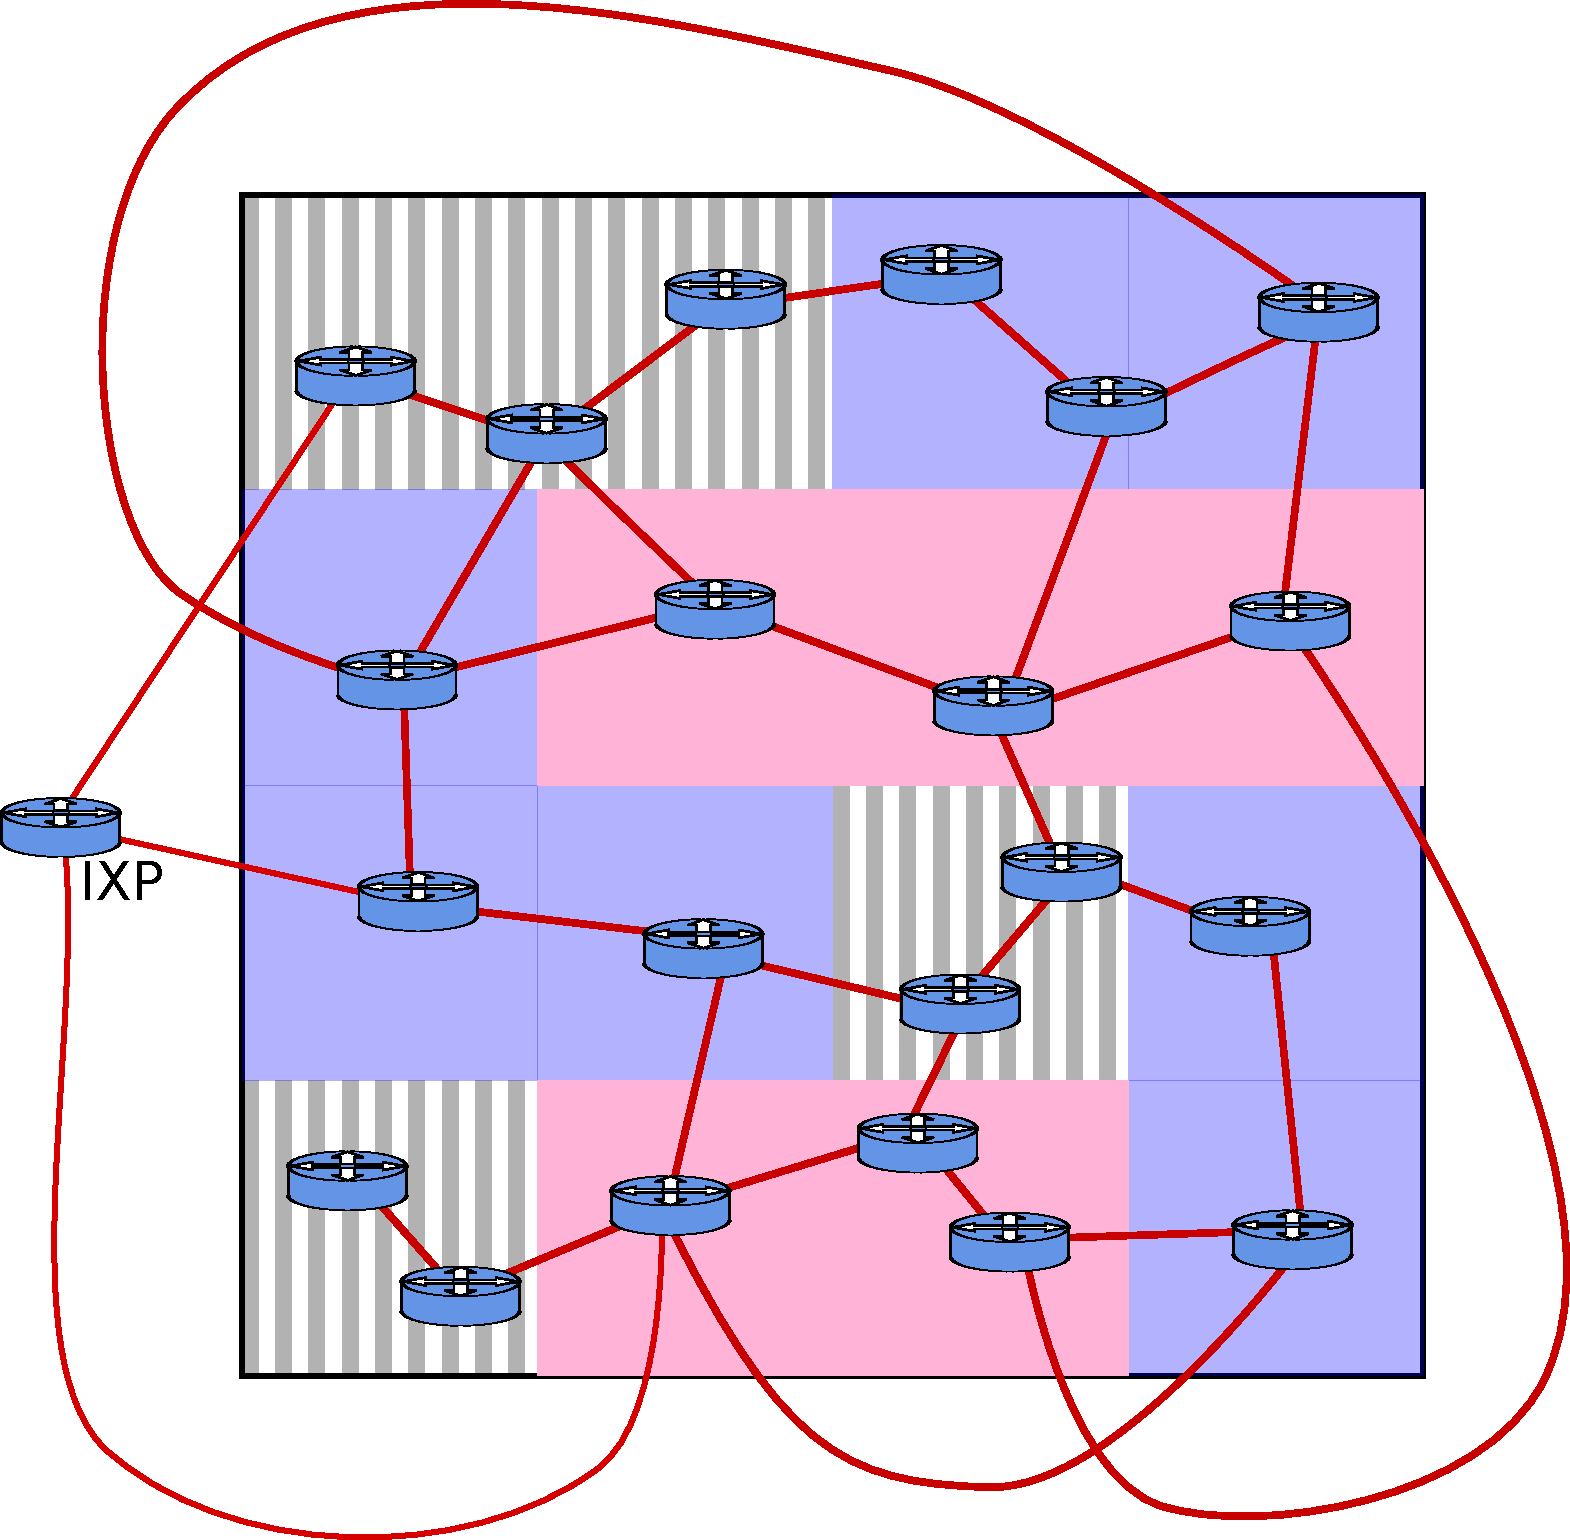
\includegraphics[width=1\textwidth]{puzzle_2.pdf}
      \caption{A possible picture of the router-level connectivity.}
    \end{subfigure}
    \caption{An illustration of the obfuscation of the AS-graph
      (in the vein of \cite{griffin02:_under_border_gatew_protoc_bgp}). The
      graph may appear simple, but hides heterogeneous, non-atomic,
      dis-contiguous entities and interconnects. At the minimum, this
      should illustrate the dangers of talking about the ``Internet''
      graph. \label{fig:puzzle}}
  \end{center}
\end{figure}         

Moreover, the AS-graph treats ASes as nodes, with connecting edges,
but the real situation is much more complex. ASes are complex networks
in their own right, and are connected sometimes by multiple edges
(M{\'e}rindol~\etal~\cite{merindol09:_quant_ases} found that
over half of the ASes they studied were connected by multiple links),
and sometimes through Internet eXchange Points (IXPs) that connect
multiple ASes. In fact, the traditional approach of modeling the
AS-level Internet as a simple connected di-graph is an abstraction
incapable of capturing important facets of the rich semantics of
real-world inter-AS relationships, including different
interconnections for different policies and/or different
interconnection
points~\cite{muehlbauer06:_build_as,muehlbauer07:_in_search}. The
implications of such abstractions need to be recognized before
attributing network-specific meaning to findings derived from the
resulting models.


% In addition to these seemingly trivial, but actually subtle and
% important points of definition, we have those of the level of
% abstraction desired:
% \begin{enumerate}

% \item The commonly-used practice of abstracting ASes to generic atomic
%   nodes without any internal structure is an over-simplification that
%   severely limits our ability to capture critical features associated
%   with real-world ASes such as route diversity, policy diversity, or
%   multi-connectivity.

% \item The traditional approach of modeling the AS-level Internet as a
%   simple connected di-graph is an abstraction incapable of capturing
%   important facets of the rich semantics of real-world inter-AS
%   relationships, including different interconnections for different
%   policies and/or different interconnection points. The implications
%   of such abstractions need to be recognized before attributing
%   network-specific meaning to findings derived from the resulting
%   models.

% \item AS topology as an uninspiring and often meaningless abstract
%   graph towards an approach that views the AS Internet as an economic
%   construct that is constrained by socio-technological factors and is
%   driven by economic incentives and business decisions made by the
%   major players in this area (\eg service and content providers,
%   large corporations, governments).  Although this notion has been
%   advanced by the networking operator community for some
%   time~\cite{norton1,norton_paid_peering,huston99:_peering_i,huston99:_peering_ii},
%   the networking research community has been slow to react and to
%   distance itself from the popular graph view of the inter-domain
%   topology (examples of exceptions
%   include~\cite{chang95,dhamdhere:conext10,labovitz10:_inter_inter_domain_traff}).

% \end{enumerate}


\subsection{Know your measurements}
\label{sec:as_measurement} 

In studying the AS-level Internet, there are some critical differences compared 
to looking at the router-level Internet:

\begin{itemize}

\item No-one ``owns'' the AS structure. There isn't anyone with the type of 
privileged view that a network operator has of its own network. There are 
tens of thousands of ASes, and so we can't reasonably expect to consult all 
of them to collate a picture either.

\item ASes are not ``nodes''. They are complex in their own right, so viewing 
the AS-level Internet as an AS-graph is a big abstraction of reality.

\item Routing between ASes is very different from routing within ASes and 
highlights the difference between graph representations that 
reflect ``reachability" vs. ``connectivity" information.

\end{itemize}

These differences create interesting problems and opportunities for
measurements, some with parallels to the router-level measurement
problems and others without any such parallels.

\subsubsection{Data-plane vs. control-plane measurements}

As discussed in \autoref{sec:router_measurements}, despite all its
deficiencies, traceroute has been the method-of-choice for obtaining
router-level measurements. As a prime example of an active measurement
tool that is confined to the data plane (\ie probe packets take the
same paths as generic data packets), traceroute has also been used to
obtain information about the AS topology but has additional problems
in this domain.

Apart from the already problematic issues (\eg load-balancing,
aliasing, missing data), IP addresses along traceroute paths must now
be mapped to ASes.  This mapping is even harder than the mapping to
routers, not just because the data for doing so is inaccurate or
incomplete (\eg IP to organization allocations may not work because
an organization does not directly correspond to an AS), but also
because the border of an AS is not well-defined in terms of IP
addresses. It is common for a link between two ASes to come from a
subnet allocated by one of the ASes, resulting in an interface in the
other network with an address that is not its
own~\cite{mao03:_as-tr,marchetta13:_detec_third_addres_tracer_traces}.
The problem is further complicated by variations such as anycast or
Multiple Origin ASes \cite{Zhao01:_MOAS}, which provide yet another
set of counter-examples to a straight-forward mapping between AS and
address space. Some work has concentrated on trying to improve the
mapping \cite{pansiot10:_extrac}, and these represent technical
advances, but it is important to understand that the fundamental
difficultly lies in the fact that the boundaries of the ``business''
are not equivalent to the AS boundaries.
 
The other major alternative to obtaining information about the AS topology is 
to collect control plane data in the form of directly measured routing information.  
The primary example of such control plane data are BGP-derived measurements. 
BGP is a path-vector routing protocol, and as such each node transmits
to its neighbors information about the {\em best} path that it knows to 
a destination. Each node then takes the information it has received about 
best paths, and computes its own best path, which it transmits to its neighbors.  
A route monitor receives this information as would any router, and from the 
transmitted path information, can infer links between ASes.  The two best known 
projects that rely on BGP route monitors, Oregon RouteViews~\cite{ORVdata}, 
and RIPE (R\'{e}seaux IP Europ\'{e}ens)'s Routing Information Service~\cite{RIPEdata} 
both use this approach, and each connects to a few dozen different ASes.

However, by its very design, BGP is an information-hiding rather than an 
information-revealing routing protocol. In addition, by its very design, 
BGP is all about reachability and {\bf not} connectivity.  Using it for 
mapping the Internet inter-domain topology is a ``hack'', and so it should 
come as no surprise that it has its own set of problems, including the following:

\begin{itemize}

\item The AS-path information in the announcements is primarily
included for loop detection and does not have to correspond to
reality. It is easy (and not uncommon) to insert additional ASes into 
a path for various purposes, \eg traffic engineering or
measurement~\cite{colitti06:_poison,bush09:_inter_optom}, and
moreover, the AS-path does not have to represent the data path.

\item Path-vector protocols do not transmit information on every path 
in the network. For instance, backup paths may never appear in any 
routing announcements (unless there is a failure), and so may not be 
seen by a route monitor.

\item Path-vector protocols only transmit ``best'' paths, and so there 
is a large loss of visibility from any one viewpoint. It is sometimes 
argued that a large number of viewpoints would
alleviate this, but the viewpoint locations are highly biased
towards larger networks, and this known ``vantage point problem" 
severely biases the possible views of the network~\cite{roughan08:_bigfoot}. 

\end{itemize}

The BGP measurement data being provided by RIPE and RouteViews was originally 
intended to help debug networks, not for mapping. While this data collections 
have been invaluable for that intended original purpose, it is unsurprising 
that it is inadequate when used for a rather different purpose such as mapping 
the AS Internet. However, when this aspect is carefully taken into account, 
good work can be done but requires a critical evaluation of the data.  Problems 
arise primarily when this data is used uncritically.  Other useful sources of 
AS-level measurements such as looking glass servers and route registries suffer 
from similar problems~\cite{Mahadevan06,he07}, and do so for similar reasons: 
they weren't intended to draw a map of the AS Internet.

\subsubsection{Attribute discovery}

The AS topology may be interesting to scientists in itself, but to be useful 
to network engineers, the routing policies that accompany it should also be known.  
It has been common to approximate the range of policies between ASes by a simple 
set of three relationships: (a) customer-provider, (b) peer-peer, and (c) siblings.  
This reduction was at least in part motivated by Huston~\cite{huston99:_peering_i,huston99:_peering_ii} and has been used in various places
\cite{subramanian02:_charac_inter,wang03:_infer,xia04:_as}.  While many 
relationships fall into these three categories, there are frequent exceptions~\cite{hyun03:_tracer_and_bgp,muehlbauer06:_build_as,Qiu07}, for instance, in the form 
of partial transit in a particular region~\cite{maz:partial-transit,norton1}.

Forgetting for the moment the simplification in assuming all policies fit this 
model and the simplifications the AS-graph itself makes, the relationships can 
be represented in the graph by providing simple labels for each edge. Typically, 
the next step after inferring network topology is to infer policies between ASes. 
The most common approach to this problem is to assume the universality of the peer-peer, 
customer-provider, sibling-sibling model, and to infer the policies by finding an 
allocation of policies consistent with the observed
routing~\cite{gao_inferring,xia04:_as,wang03:_infer,battista_inferring:2003,dimitropoulos07:_as_relat}. 

Once relationships are established, a seemingly reasonable next step
is to estimate the hierarchical structure as in
\cite{subramanian02:_charac_inter}. However, the effect of large
numbers of (biased) missing links has not really been considered in
these algorithms.  In fact, the tier structure of the Internet seems
to be largely an illusion. Recent work has shown that there is little
value in the model at
present~\cite{gill08:_flatt_inter_topol,labovitz10:_inter_inter_domain_traff};
but, in contrast to the claims of these papers, there is no strong
evidence that the situation has actually changed or that the tier
model was ever a good model (except maybe in the early stage of the
``public" Internet in the latter 20th century) particularly in light
of the problems in the data.

Alternatively, we can infer a generic set of policies consistent with
routing observations using a more detailed set of routing
measurements~\cite{path_inference_sigmetrics:2005,muehlbauer06:_build_as}
and estimate performance by comparing predicted routes to real routes
(held back from the inference process).


\subsubsection{The ``missing link" problem: Extent and impact}

Perhaps the most obvious problem that results from relying on BGP measurement 
data to map the AS-level Internet is that there are many missing links in the 
resulting AS-graph.  To illustrate the extent of this problem, years of 
concentrated research efforts that relied on a combination of improved inference methods and additional data sources~\cite{chang04:_towards,zhang05:_collec_inter_as_topol,muehlbauer06:_build_as,dimitropoulos07:_as_relat,he07,he09:_lord_of_links,roughan08:_bigfoot,augustin09:_ixps,chen09:_sidewalk,oliveira10:_incompl_of_obser_inter,dhamdhere11:_twelv_years_evolut_inter_ecosy,sanchez13:_dasu}
have produced a picture of the Internet's AS topology that --- as of 
2011 --- consisted of some 35,000-40,000 ASes (nodes) and about 115,000-135,000 
edges (AS links), with about 80,000-90,000 of them being of the customer-provider type and 
35,000-45,000 of the peer-peer type.

More recently, this supposedly up-to-date and most complete view of
the AS-level Internet changed drastically thanks
to~\cite{ager12:_anatom_europ_ixp} that relied on ground truth data
from one of the largest IXPs in Europe (and worldwide) that had at the
time of this study almost 400 member ASes. The main finding of this
recent study is that in this single location, the number of actively
used AS links of the peer-peer type was more the 50,000 --- larger
than the number of all AS links of the peer-peer type in the entire
Internet known as of 2011. Moreover, being extremely conservative when
extrapolating from this IXP to the Internet as a whole,
\cite{ager12:_anatom_europ_ixp} shows that there are easily more than
200,000 AS links of the peer-peer type in the entire Internet, more
than twice the number of all AS links of the customer-provider type
Internet-wide.  Importantly, the main reason for this abundance of AS
links of the peer-peer type at IXPs is well understood --- many IXPs,
especially the larger ones, offer as free service to their member ASes
the use of their route server. This service greatly facilitates the
establishment of peer-peer links between the members of an IXP and has
become enormously popular with members that have an ``open" (as
compared to restrictive or selective) peering policy. Especially for
the larger IXPs, such networks typically constitute the vast majority
of IXP member ASes. \autoref{fig:ixp} provides an illustration of the
connectivity through this IXP and shows that a majority of its member
ASes have an open peering policy (some 300+ members) and establish AS
links of the peer-peer type with one another.

\begin{figure}[thbp] 
  \begin{center}
% pdfimages gets actual 'images' (bitmaps) out of the PDF, but not plots
%  pdfjam p163-ager.pdf  '7' --outfile p163-ager-p7.pdf 
%     extracts a particular page so I can use it here
    \includegraphics*[width=0.65\columnwidth,viewport=77mm 225mm 133mm 270mm]{p163-ager-p7.pdf}
%                                                    xleft ybottom xright ytop
%                                                 a4 = 0 0 210 297
    \caption{Scatter-plot of number of peers per member, based on a
      classification of the member ASes in the four business
      categories defined above: LISP (Large ISP), SISP (Small ISP),
      HCDN (Hosting/service and Content Distribution Network)), and
      AEN (Academic and Enterprise Networks), and by tier.  
      (Reprinted from \cite{ager12:_anatom_europ_ixp}; \copyright 2012 ACM, Inc. Included here by permission.)
      \label{fig:ixp}}
  \end{center}
\end{figure}         

In short, for many years, researchers have worked with AS-graphs that are typically complete 
in terms of nodes, but easily miss more than half the edges. Importantly, these graphs 
have generally a 2:1 ratio of customer-provider type vs. peer-peer type links when 
a 1:3 ratio is much more likely to reflect Internet reality. Clearly, for gaining 
any economic-based understanding of the AS Internet, getting that ratio approximately 
correct is paramount because it is directly impacting how money flows in the 
Internet --- while in a customer-provider relationship, the former pays the latter 
for bandwidth, peer-peer relationships are typically settlement-free (\ie no 
money is exchanged between the involved parties).  

Besides their immediate economic impact, the above missing edges cause also 
significant problems in inferring the AS graph. For instance, it is a requirement 
that a network be multi-homed to obtain an ASN. This means the AS needs to intent 
to connect to at least two upstream providers. In this sense a ``single-homed stub-AS''
does not exist.  Without any doubt, there are exceptions to this rule. However, the 
second link is often a backup link which is invisible to BGP outside of the immediate 
connection, because of BGP's information hiding\footnote{Note that complex BGP policies 
may play a role in this as well~\cite{cost_community,tim:wedgies}.}. Thus, it may 
appear as if a large number of ASes are single-homed stubs.

In \cite{oliveira10:_incompl_of_obser_inter}, the authors separate the missing 
links into {\em hidden} and {\em invisible}.  Whereas the latter are links that 
are missing from the data for structural reasons (\ie it is not just a question 
of quantity (\ie numbers of monitors) but quality (\ie location of monitor)), 
the {\em hidden} links may be found with enough measurements (over time, or 
multiple viewpoints). In \cite{roughan08:_bigfoot} the authors extend that by 
dividing links into a number of classes based on their observability.

The ``missing link" problem in the AS context is much more serious than if those 
links were ``missing at random''.  In particular, the bias in the type of links 
that are missing~\cite{roughan08:_bigfoot} is critical when calculating some 
metrics on the graph, such as distances, precisely because such links are often 
{\em designed} to cut down on the number of ASes traffic must traverse. The 
missing data is also crucial for understanding reliability: for instance, papers 
such as \cite{barabasi00} that argue that high-degree nodes create
vulnerabilities in the Internet ignore the backup links that are invisible in 
these dataset, but obviously crucial when studying the resilience of the network.

\subsection{The Internet's AS-level topologies}

Despite the limitations of measurements, there is a considerable
amount known about the AS-level topology of the Internet, and we talk
here about the issues in defining and modelling that topology.  We
have seen that the definition of an AS is fraught with
problems. Assuming for the time being that the concept of an AS is
well defined so that it makes sense to equate each AS with a node in a
graph, then what is the set of links?  Unfortunately, the question of
which ASes are ``adjacent'' also has no simple answer, and defining
the meaning of a ``link'' between two ASes requires further
consideration.

Does a link mean the ASes have a business relationship, physical
connectivity, connecting BGP session, or that they share traffic? All
the above are reasonable definitions, and none are equivalent. A
common definition is that two ASes are said to be connected (at a
particular time), if they can exchange routing data (and presumably IP
traffic) without the help of an intermediary AS that provides {\em
  transit}. However, this says little about the true business
relationships that are sometimes discussed as a matter of course when
the AS-graph is considered. Moreover, this abstraction looses
considerable information. In reality there are multiple topologies we
want to model, each with its own meaning, structure, potential
applications, and inference problems.

\begin{itemize}

\item {\em Business relationship graph:} in its simplest form this
  graph simply indicates (by an edge) that a business relationship
  exists between the corporations that own two ASNs. Edges could be
  usefully labelled by the type of business relationship, and we list
  a small subset of the possible relationships in
  \autoref{tab:as_graph_set}.

\item {\em Physical link-level graph:} this graph indicates whether
  two ASNs have a physical (layer 1) connection, and how many such
  connections they have. The multiple nature of such connections leads
  this to being a multigraph, as it is very common for two ASes to be
  connected by multiple links and in different geographic locations
  \cite{norton_paid_peering,liljenstam03:_devel_of_inter_backb_topol,spring03:_inflation}. 
  The idea is clearly illustrated by Figure~1 in
  \cite{liljenstam03:_devel_of_inter_backb_topol}, which shows a
  ``pancake'' diagram of the North American Internet backbone. Perhaps
  the reason this critical aspect of the topology is typically ignored
  is that it is very hard to measure---BGP monitor data is in general blind
  to this facet of the topology.
% Traceroutes can show more detail, but suffer from their own problems.
  In addition, this graph should really be a hypergraph. A single
  ``edge'' can connect multiple ASes, for example through an IXP
  \cite{hyun03:_tracer_and_bgp,xu04:_ixps,augustin09:_ixps}. One might
  argue that they are joined by a switch/router, each using
  point-to-point links, but in at least some cases, that switch has no
  place in a AS graph (\ie it has no ASN).  The graph's edges could
  be usefully annotated with link capacity and potentially other
  features such as geographic location.

\item {\em Connectivity graph:} this graph indicates that layer-2
  connectivity exists between two ASNs. In many cases the layer-2
  connectivity between ASNs would be congruent with the layer-1
  connectivity, but with recent advances in network virtualization this
  may not hold for long~\cite{vroom}. 

\item {\em BGP routing graph:} the edges in this graph indicate pairs
  of ASes that have an active BGP session exchanging routing
  information (\ie a BGP session that is in the `established' state~\cite{RFC4271}).

\item {\em Policy graph:}  the edges in this graph are the same as
  those in the BGP routing graph, but include directed policy
  annotations~\cite{tim10:ssp}. We define this separately from the BGP routing graph
  because it may require a multigraph to allow for policy differences
  between different regions. 

\item {\em Traffic graph:} it is the same as the BGP routing graph,
  but the edges are annotated with the amount of traffic exchanged
  between the corresponding ASes.

\end{itemize} 

This is hardly a complete set of possibilities, but already we can see
the potential complexity here. Nevertheless, it appears unusual for studies to
even define precisely what graph they examine (exceptions being papers
such as \cite{govindan97:_topology,oliveira10:_incompl_of_obser_inter}
where the BGP routing graph is explicitly considered).  In
\autoref{tab:as_graph_set}, we list some of the possible graphs, and
their basic properties.  There is no clean 1:1 mapping between
``network'' and ``organization'' and ``AS''
\cite{hyun03:_tracer_and_bgp,cai10:_AS_to_organ_map}, and so it is
highly non-trivial to map between these graphs, and they are certainly
not equivalent.


\begin{table*}[t]
\begin{center}
  \begin{tabular}{|l|l|l|}
    \hline 
    Graph & Edge Annotation & Graph Type \\
    \hline 
    business relationship & subsidiary, partner, customer,... & directed graph \\
    physical link-level & link capacity & multi- hyper-graph \\
    connectivity graph & - & multigraph \\
    BGP routing graph & - & undirected graph \\
    policy graph & BGP policies & directed multigraph \\
    traffic graph & traffic volumes & directed graph \\
     \hline 
  \end{tabular}
  \caption{Example elements of the set of AS graphs.}
  \label{tab:as_graph_set}
\end{center}
\end{table*}


% It should also be clear by now that ASes are not atomic, they are
% geographically distributed entities \cite{rasti10:_eyebal_ases},
% comprised of multiple components distributed over some area of
% space. In principle (according to the RFCs) the AS should have one
% routing policy. Not only is it not exactly clear what this means, but
% it is clearly not
% true~\cite{hyun03:_tracer_and_bgp,muehlbauer06:_build_as,bush09:_inter_optom}.
% The components of an AS may not even be contiguous. An AS may rely on
% a provider AS for transit of its traffic between multiple otherwise
% disconnected components.


\subsection{A look ahead}

Given our list of problems described here, one might be tempted to
think that the AS-graph and routing data in general are useless until
these datasets are drastically improved. However, apart from their
operational utility, RouteViews and RIPE RIS have provided the
essential ingredients for many important studies that match those
services' goals~\cite{RISgoals}. A number of these studies have
improved the Internet significantly, and in the majority of such
successful papers there is no need to exploit the ``graph'' view of
the network. Examples include: (a) The discovery of slow convergence
and persistence oscillation in routing
protocols~\cite{varadhan96:_oscillation,labovitzSig97,labovitzInfo99,labovtizFTCS99,labovitzSig00,govindanNetworks00,griffin02:_analy_med_oscil_probl_bgp}. (b)
Understanding of the impacts (positive and negative) of route flap
dampening~\cite{mao02:_flap,pelsser:rfd}. (c) Determining how much
address space and how many ASNs are being actively
used~\cite{address_space_growth}. (d) Looking for routing ``Bogons''
often related to Internet address hijacking
%\footnote{Hijacking is becoming a potentially destructive problem. See the recent incident with China Telecom \cite{chinahijacking}.}
\cite{ramachandran06:_spam,cymru,hijacking,nick-bogon,chinahijacking}. (e) Debugging
network
problems~\cite{bush07:_testin,feldmann04:_bgp,roughan04:_SNMP_BGPb}.

On the measurement side, there have also been many advancements
towards improving our view of AS topology. For instance:

\begin{enumerate}

\item As BGP routing changes, often
  multiple potential paths are explored and these paths (which are
  unlikely to actually be used as a final choice) can show some of the
  alternative routes available in the
  network~\cite{zhang05:_collec_inter_as_topol}, and thus a more
  complete topology.

\item Missing edges can be found using additional datasets, \eg RIRs
  and looking glasses~\cite{chang04:_towards,zhang05:_collec_inter_as_topol,he07,he09:_lord_of_links},
  or IXP data~\cite{he07,he09:_lord_of_links,augustin09:_ixps,sanchez13:_dasu},
  though care must be exercised with any additional dataset.

\item A routing beacon~\cite{labovitzSig97,mao03:_bgp_beacon,bush09:_inter_optom}
  is just a router that advertises and withdraws
  certain prefixes on a regular schedule. Examination of the observed
  announcements and withdrawals by various route monitors then allows
  estimates of protocol behavior such as convergence time. 

\item Route poisoning prevents announcement from reaching
  certain parts of the Internet. As with beacons, it allows one to
  examine the behavior of BGP in a more controlled manner. This is perhaps 
  the only way to see (some) backup paths, or to understand whether an ISP uses default
  routing~\cite{colitti06:_poison,bush09:_inter_optom}.

\item There are also attempts to not just estimate the topology
  but derive some quality measure for the resultant
  AS-graph~\cite{inter_as_level_topol_const_analy,winter09:_model_inter_routin_topol_with,roughan08:_bigfoot}.
 
\end{enumerate}

There is often an unfortunate side-effect to some of these types of measurement in
form of a Heisenberg-like uncertainty principle. That is, it is not clear
whether observed changes are due to the micro-phenomenon of path
exploration or macro-phenomena of link changes, new entrants, etc.
The longer we make observations, the more complete they may seem,
but we then do not know whether all of those links existed at the
same time. Such uncertainty principles appear to be present in a
number of Internet measurement contexts~\cite{roughan05:_fundamental} 
where we trade off ``accuracy'' of the measurements against ``time localization''.
In any case, this approach does not overcome the structural bias mentioned earlier. 

At the same time, the above-mentioned and other advances on the measurement side
suggest that the missing link problem may be improved, providing
``more complete'' AS graphs. However, there is a profound need
(illustrated by the above) for better data accuracy measurements, and
better response to data quality issues from subsequent users of the
data. Obvious ways to improve are to conduct sensitivity analysis (of
results) to missing or incorrect input data. 

In addition, it is to be hoped that more controlled experiments are
conducted (\ie experiments that have a ``control'' sample against
which the experimental data can be compared) in order to precisely
derive which factors of interest affect which variables.  Controls
allow one to discriminate alternative explanations for results, and
prevent the affects of one confounding factor drowning out the affects
of others (see \cite{mao03:_bgp_beacon,bush09:_inter_optom}). This is
basic tenet of the scientific method, but seems to have been ignored
in this area of research. Most studies have been ``observational'',
and while there is a valid role for such experiments, for instance in
epidemiology, they are intrinsically harder to interpret.

Lastly, another aspect of this richer set of AS topologies is that it should be
obvious by now that economic or commercial objectives by and large determine
and shape the structure and evolution of their real-world counterparts, and that 
these constructs are once again naturally expressed through optimization rather 
than random graph models, though in this case the optimization problems may come
from game theory or economics rather than mathematical programming. 

\subsection{Notes}

The primary sources for the material presented in this section are

\begin{itemize}

\item[\cite{roughan11}] M. Roughan, W. Willinger, O. Maennel,
D. Perouli, and R. Bush. 10 Lessons from 10 Years of Measuring and Modeling the Internet's Autonomous Systems, in: {\em IEEE Journal on Selected Areas in Communications} 29(9):1810-1821, 2011.

\item[\cite{ager12:_anatom_europ_ixp}] B. Ager, N. Chatzis,
A. Feldmann, N. Sarrar, S. Uhlig, and W. Willinger. Anatomy of a
large European IXP, in: {\em Proc. ACM SIGCOMM'12, ACM Computer
Communication Review} 42(4), 2012.

\end{itemize}
and they contain lengthier discussions of many of the issues touched upon here. 

For additional and more in-depth reading materials (in
addition to the references indicated throughout) we point to

\begin{itemize}

\item[\cite{chang-thesis06}] H. Chang. Modeling the Internet's
Inter-Domain Topology and Traffic Demand Based on Internet Business Characterization, PhD Thesis, University of Michigan, 2006.

\item[\cite{Donnet07}] B.Donnet and  T. Friedman, Internet Topology Discovery: A Survey, IEEE Communications Surveys \& Tutorials, 9(4), pp.56-69, 2007.

\item[\cite{dhamdhere-thesis08}] A. Dhamdhere. Understanding the
Evolution of the AS-level Internet Ecosystem, PhD Thesis, Georgia Institute of Technology, 2008.

\item[\cite{haddadi08:_networ_topol}] H. Haddadi, M. Rio,
G. Iannaccone, A. Moore and R. Mortier, Network topologies:
inference, modeling and generation, IEEE Communications Surveys,
10(2), 2008.

\item[\cite{dhamdhere11:_twelv_years_evolut_inter_ecosy}] A. Dhamdhere
  and C. Dovrolis. Twelve Years in the Evolution of the Internet
  Ecosystem, in: {\em IEEE/ACM Transactions on Networking} 19(5),
  2011.

\end{itemize}
